
\subsection{Transforming the Network}
There are three types of operation which we can perform upon our network.
We’ll introduce three steps involving these.
\newpage
\noindent\textbf{Step 1} We start by looking at the polygonal faces of the network and ask: is there a face with more than three sides? If there is, we draw a diagonal as
shown in the diagram below, splitting the face into two smaller faces.

\begin{figure}[h]
	\centering
	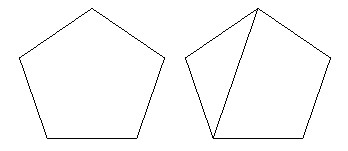
\includegraphics[width=0.8\linewidth]{images/dividing_faces}
	\caption{Dividing faces}
\end{figure}

We repeat this with our chosen face until the face has been broken up into
triangles.

\begin{figure}[h]
	\centering
	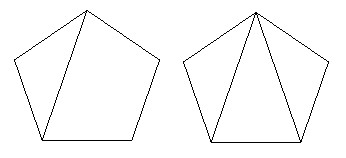
\includegraphics[width=0.8\linewidth]{images/triangular_faces}
	\caption{In the end we are left with triangular faces.}
\end{figure}

If there is a further face with more than three sides, we use Step 1 on that
face until it too has been broken up into triangular faces. In this way, we can
break every face up into triangular faces, and we get a new network, all of
whose faces are triangular. We illustrate this process by showing how we would
transform the network we made from a cube.

We go back to \textbf{Step 1}, and look at the network we get after performing
\textbf{Step 1} just once. Now, by drawing a diagonal we added one edge. Our original
face has become two faces, so we have added one to the number of faces. We
haven’t changed the number of vertices. The network now has $V$ vertices, $E + 1$
edges and $F + 1$ faces. So how has $V - E + F$ changed after we performed \textbf{Step 1} once? Using what we know about the changes in $V$ , $E$ and $F$ we can see that


\begin{figure}[h]
\centering
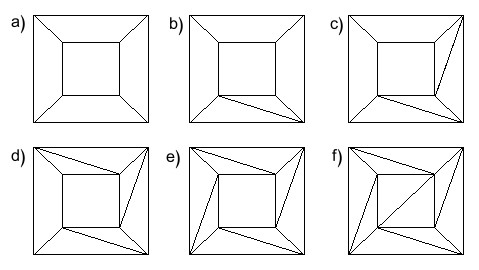
\includegraphics[width=1 \textwidth]{images/cube_triangular_faces}
\caption{This is what happens to the cube’s network as we repeatedly perform \textbf{Step 1.
}}
\end{figure}

\noindent {}${\text{V - E + F}}$ has become ${\text{V - (E+1) + (F+1)}}$. Now we have: \\
\begin{equation}
V - (E+1) + (F+1)= V - E - 1 + F + 1 = V - E + F
\end{equation}


\noindent So ${\text{V - E + F}}$ has not changed after \textbf{Step 1}! Because each use of \textbf{Step 1} leaves
${\text{V - E + F}}$ unchanged, it is still unchanged when we reach our new network
made up entirely of triangles! The effect on ${\text{V - E + F}}$ as we transform the
network made from the cube is shown in the Table ~\ref{tab:Euler law}.

\begin{table}[h!]
	\begin{center}
		\caption{Steps of the Euler law derivation.}
		\label{tab:Euler law}
		\begin{tabular}{| c | c | c | c | c |}
			\hline
			Round & $V$ & $E$ & $F$ & $V-E+F$ \\ \hline
			(a) & 8 & 12 & 6 & 2 \\ \hline
			(b) & 8 & 13 & 7 & 2 \\ \hline
			(c) & 8 & 14 & 8 & 2 \\ \hline
			(d) & 8 & 15 & 9 & 2 \\ \hline
			(e) & 8 & 16 & 10 & 2 \\ \hline
			(f) & 8 & 17 & 11 & 2 \\ \hline
		\end{tabular}
	\end{center}


\end{table}

